% Created 2018-04-27 Fri 14:02
\documentclass[12pt, letterpaper]{paper}
\usepackage[utf8]{inputenc}
\usepackage[T1]{fontenc}
\usepackage{fixltx2e}
\usepackage{graphicx}
\usepackage{longtable}
\usepackage{float}
\usepackage{wrapfig}
\usepackage{rotating}
\usepackage[normalem]{ulem}
\usepackage{amsmath}
\usepackage{textcomp}
\usepackage{marvosym}
\usepackage{wasysym}
\usepackage{amssymb}
\usepackage{hyperref}
\tolerance=1000
\usepackage{minted}
\usepackage{natbib}
\usepackage[margin=1in]{geometry}
\def\BigO{{\cal O}}
\renewcommand\maketitle{}
\author{Timothy Schwieg}
\date{\today}
\title{An Application of Cumulative Prospect Theory to Online lotteries in Counter-Strike: Global Offensive}
\hypersetup{
  pdfkeywords={},
  pdfsubject={},
  pdfcreator={Emacs 25.3.1 (Org mode 8.2.10)}}
\begin{document}

\maketitle
\bibliographystyle{chicago}

\begin{titlepage}
\centering
{\scshape\LARGE University of Chicago Economics Department\par}
\vspace{1cm}
{\scshape\Large Writing Sample\par}
\vspace{1.5cm}
{\huge\bfseries An Application of Cumulative Prospect Theory to Online lotteries in Counter-Strike: Global Offensive\par}
\vspace{2cm}
{\Large\itshape Timothy Schwieg\par}
\vfill
Originally Submitted as a term paper for ECO 6315 Current Seminar in Economic Topics
\vfill

{\large \today\par}
\end{titlepage}

\section{Introduction}
\label{sec-1}
A common criticism of neo-classical economics is the structure that is
placed on actions taken by agents under risk. Often times economists
assume that agents act to optimize expected utility, where the utility
is characterized by a Von-Neumann Morgenstern utility function. This
has many attractive properties, but can lead to situations where the
structure is too rigid to allow for commonly observed behavior.

One such example is lotteries. People who are generally risk-averse in
areas such as insurance act as if they are risk-loving in playing a
lottery. One model that is able to account for this is cumulative
prospect theory. It incorporates several important concepts not seen
in classical decision making under risk.

It incorporates reference dependence, which implies that people view
things in the context of losses and gains rather than changes to their
overall wealth. This is attractive for computational reasons. It also
utilizes loss aversion, the notion that losses are relatively more
costly than gains. The model also incorporates diminishing
sensitivity, the notion that valuations are concave in losses and
convex in gains. The final concept is probability weighting, the
notion that consumers act as if they were facing different
probabilities than what they encounter.

The nature of probability weighting leads to an overweighting of the
tails of the distributions. This can cause behavior such as preferring
a 0.001 chance of \$5000 to a certain gain of \$5, and simultaneously
preferring a certain loss of \$5 to a .001 chance of losing \$5000. As
noted by \cite{LitReview}, there have been more sophisticated approaches
to the application, however this investigation will be limited to the
relatively simple functional forms suggested first by \cite{Kahn}. This
was chosen due to the computationally arduous estimation method
utilized.

In this paper I apply cumulative prospect theory to small lotteries
that take place within the video game \emph{Counter Strike: Global
Offensive}. In this game players receive "loot boxes", which are cases
that can be opened with the purchase of a key and return a random
reward based on some well-known probabilities. There is a well defined
market for cosmetic items, taking the form of a continuous
double auction where players can buy and sell virtually all items in
the game. There is a large number of items sold daily at non-trivial
prices, so the data is a powerful framework for investigating consumer
behavior under lotteries.

A very attractive feature of this data is that both the contents of
the lottery and the lotteries themselves are both traded on the Steam
Community Market. While the API does not provide flawless data, there
is still a large amount of data. This comes in two forms: Market
history given to the last hour, and Buy and Sell Orders that have not
currently been fulfilled.

I will test if the data gathered from the steam community market
is consistent with the predictions of cumulative prospect theory, as
well as look at how the different structures of the lotteries
affect the way in which consumers treat the lotteries. In particular,
I am interested in testing whether or not loss aversion is present in
this data, and whether or not several of the lotteries which have many
more low probability but very high value items have different valuation
functions compared to the other lotteries.

\section{Model}
\label{sec-2}
\subsection{General Approach}
\label{sec-2-1}

Because of the nature of the data, as well as the complicated
structure that cumulative prospect theory places upon the valuation
function, it is difficult to implant it within the structure used
commonly in double auction literature. Almost all models of auctions
specify a structure between the valuation and the price that is the
valuation for the item minus the price paid for the item at the
auction. This difference cannot be reconciled with the framing effects
required by cumulative prospect theory.

This forces us to take a relatively agnostic take on the structure of
the model. Since the valuations of every consumer are not observed, we
only observe purchases made, we know that the valuation of the buyer
must be at or above the price of the item. One powerful result shown
by \cite{Efficiency} is that will drive all the computations of the
model is that a continuous double auction converges in order $\BigO (
N^2 )$ to a competitive market. From this, I can consider that in large
double auctions, such as the case for the data present, that we are
working in a competitive market. From this we can conduct our analysis
as if a buyer of a lottery is at a competitive market, sees the price
given by the market exogenously, and makes a decision choice based
upon his valuation as a function of the price. While there is not
nearly enough information given to be able to identify supply and
demand within this market, we are only interested in the valuations of
the purchasers of the lotteries, and we may approach this by
considering a single buyer who has independently formed a private
valuation of the lottery and enters the market.

Since there is a  large number of consumers in the market, we may take
price as exogenous. Since the order of the covariance between the
price and the valuations is $\BigO ( \frac{1}{N} )$. The differences
between the competitive market and the double auction become
meaningless since the double auction is converging at a much faster
rate to the competitive market. That is, even if the order of the
covariance was higher for a double auction, we are converging to a
competitive market so quickly we can effectively consider the market
fixed at a competitive market and then consider the covariance between
price and valuations. Due to the large magnitude of the data being
examined, the price is effectively independent of an individuals
valuation, so the assumption of exogenous prices is reasonable, and
will drive much of the computation throughout the paper.

This leads us to one of two outcomes in the market, either there is a
purchase made, indicating a valuation above the price seen by the
consumer, or he leaves a buy order, indicating a price he would be
willing to pay. The structure of the double auctions is such that the
buyer pays the seller's price, not his valuation. Since in a double
auction where the buyer pays the seller's price, \cite{PriceDataOnly}
has shown that it is dominant to tell the truth. As a result I will
consider these buy orders as the actual valuations of the
consumer. This means that while the data taken at market is censored
by the market price, the data taken from the buy orders is not, and
our model will have to encompass both forms.


\subsection{Discrete Choice}
\label{sec-2-2}
There is no data on the consumers purchasing the items, and we only
have data on a single item being purchased rather than consumers
facing bundles of possible items in $\mathbb{R}^n$ such as consumer
theory would ordinarily predict. These two results mean that we must
work within a framework of making a single decision to purchase the
lottery or not, and with relatively little structure so as to support
the complex structure of cumulative prospect theory. One such model is
Discrete Choice theory.

By Following the discrete choice model, we assert that decisions made
by the individual are made such that if the valuations of lottery plus
$\xi_l$ is greater than the valuation of not purchasing which is given
by $\xi_n$ where $\xi$$_{\text{j}}$ $\sim$ Gumbel. This means that the purchase is
dictated by if: $V(f) + \xi_b - \xi_n > 0$. Since the difference of
two Gumbel distribution is distribution logistically, and V(f) is not
random. Knowing that the Logistic Distribution is in the location
scale family, we may consider the entire expression as: $V_i(f) \sim
logit( V(f), s )$.

However, we observe some censored realizations of V. That is, we
observe valuations based on the buy orders which are non-censored
realizations, but we also observe purchases which are censored. Denote
the censored purchases by $d_n = 1$ and uncensored by: $d_n = 0$. The
logarithm of the likelihood function for censored data as shown by
\cite{LimeBoy} is:

\begin{equation}
\label{Likelihood}
\sum_{j=1}^J \sum_{n=1}^{N_j} d_{n,j} \log( \frac{1}{4s} sech^2 ( \frac{x_{n,j} - V_j}{2s} ) ) + (1-d_{n,j}) \log ( \frac{\exp(\frac{x_{n,j} - V_j}{s})}{1+\exp(\frac{x_{n,j} - V_j}{s})} )
\end{equation}

Where $V_j$ is the valuation for the box of type j, x$_{\text{n,j}}$ is the price
paid by observation n of type j, and d$_{\text{n,j}}$ is whether or not the data
at observation n of type j was censored.

We may maximize this log-likelihood to find the parameters that best
fit. What remains to be decided is the form of the function V. We will
have to assume a structural form for the function, and while we will
be able to compare between different structural forms, we cannot apply
any statistical tests between our different assumptions. 

\subsection{Cumulative Prospect Theory}
\label{sec-2-3}
Since one key aspect of cumulative prospect theory is that we are more
strongly motivated by losses than by gains, it is immediately obvious
that the value function of the contents of the lottery will not be
symmetric. The easiest way to handle this asymmetry will be to
estimate two separate functions, one of which is used to evaluate
losses, and one of which estimates gains. By applying a piecewise
function, we can still arrive at a continuous function (where both are
zero at zero) which we can use. The question of whether or not loss
aversion will be displayed however, is one for the data to answer.

Since I am following the Discrete Choice model, the decision to
purchase a create will be driven by the valuations of the crate
against the alternative which is buying nothing. Since Cumulative
prospect theory functions by looking at deviations from a reference
point, which we will use as the price of the box combined with the
costs of opening it (the key). Later in the analysis, this will be
relaxed, and compared against several different reference points. As
noted in \cite{LitReview}, the question of the proper reference point is
actively debated, so we will examine different possibilities.

Following the Notation of \cite{Kahn}, we represent the valuation of the
lottery as $V(f) = \sum_{i=-m}^n \pi_i v(x_i)$ where v is a function
that is convex in losses and concave in gains. $\pi$ is the weights
applied to each item in the lottery, and will not necessarily be their
actual probabilities.

In this paper, the effects of dynamics will not be considered. There
is a common pattern of the price of lotteries decreasing over time,
and there are few covariates available. Because of these two concerns,
I will not consider purchases of the boxes intended as an investment
rather than to be opened. This simplifying assumption will mean that
the valuations of the contents of the lottery drive the value, and I
believe it is reasonable based upon the price histories
available. Without this, there is not enough data available to attempt
to explain valuations of the boxes, and the dynamic nature of the
problem would increase the complexity immensely.


\subsubsection{Valuations}
\label{sec-2-3-1}
The question of how do we measure the gains of the lottery now
looms. Since each box contains an item that has a particular value to
the consumer who opened it, and is unobserved, the only thing that can
be observed is the market price of the item over time. Identification
of buyer and seller valuations, even in a simplified situation where
there is only one buyer and one seller, still requires more
information than we are given. As shown in \cite{NonParIdent}, for their
identification strategy, all the bids in the auction are required, and
for the strategy shown in \cite{PriceDataOnly}, there must exist
exclusive covariates that shift only one trader's value distribution,
which are not given by the data. Absent an ability to identify the
valuations of the specific losses and gains in the lottery, I will
have to assume that the market value of each item represents its value
to the consumer. Any item obtained in the box could in theory be
sold at the market value of the item, so we will consider this the
value for each item. 

The valuations of the i$^{\text{th}}$ possible element of the lottery will be
given by: v( p$_{\text{i}}$ - p$_{\text{l}}$ - p$_{\text{key}}$ ), where p$_{\text{i}}$ is the average price of the
i$^{\text{th}}$ element at market, p$_{\text{l}}$ is the price paid for at market for the
lottery, and p$_{\text{key}}$ is the price of the key required to open the
lottery. Depending on whether or not this difference is positive or
negative will result in different functions being used to evaluate the
valuation. Using the specification suggested by \cite{Kahn}:

\begin{equation}
\label{piecewiseValuation}
v(x) = \begin{cases} x^\alpha \quad &x \geq 0\\ -\lambda(-x)^\alpha \quad &x < 0 \end{cases}
\end{equation}

\subsubsection{Probability Weighting Function}
\label{sec-2-3-2}

In cumulative prospect theory, the cumulative mass (distribution)
function is weighted such that individuals overweight the tail
probabilities. This is especially important in this model, as there are
many high valued rare items, that if this part of the theory is
correct, heavily influence the valuation of the box, despite their
extremely low probability of occurrence.

Again, I will use the specification suggested by \cite{Kahn}, and use
the cumulative transformation function of:

\begin{equation}
\label{weightFunction}
w(P) = \frac{ P^\delta }{( P^\delta + (1-P)^\delta )^{\frac{1}{\delta}}}
\end{equation}

To define the decision weights $\pi$$_{\text{i}}$, we must first order the prospects
of the lottery in ascending order of gains. the weight $\pi$$_{\text{i}}$ then is
defined by:
\begin{equation}
\label{piWeights}
\pi_i = w( \sum_{j = -m}^i P(x_j)) - w( \sum_{j=-m}^{i-1} P(x_j) )
\end{equation}

\subsubsection{The Valuation Function}
\label{sec-2-3-3}

From these, we can create a valuation function for an individual
facing a particular lottery:
\begin{equation}
\label{Valuation}
V_i = \begin{cases}
(w( \sum_{j = -m}^i P(x_j)) - w( \sum_{j=-m}^{i-1} P(x_j) ))(p_i - p_l - p_{key})^\alpha \quad &(p_i - p_l - p_{key}) \geq 0 \\
-\lambda(w( \sum_{j = -m}^i P(x_j)) - w( \sum_{j=-m}^{i-1} P(x_j) ))(p_l + p_{key} - p_i)^\alpha \quad &(p_i - p_l - p_{key}) < 0 \\
\end{cases}
\end{equation}


\section{Data}
\label{sec-3}
\subsection{The Data}
\label{sec-3-1}
The data is price data of items on the Steam Community Market for
the game \emph{Counter Strike: Global Offensive}. Players in game earn items
random that they can sell on the market or open themselves. However
most rare items are earned via opening of dropped "loot boxes" that
are then opened by players via purchasing of a key. These boxes can be
earned by playing or received randomly from players who are watching
games of professionals play. The probabilities of the drops are not
known or even estimated well, as they change depending on many factors
including time.

However, once a box has been obtained, the probability of receiving an
item is well documented as required by Chinese Law. Each item has a
certain grade of rarity, for example the Ak-47 Redline has a rarity
level of Classified which means that there is a 3.2\% chance of
receiving a Classified item in the crate. All Classified items
contained in the crate have the same probability of being dropped by
the crate.

However there are many variants of each item. Each item has a quality
ascribed to it, the float of the item. This describes the wear on the
item, and is distributed uniformly on the interval 0-1. On the market
the items are split into intervals: Battle-scared, well-worn,
field-tested, minimal wear and factory new. Each quality is a separate
listing on the market with a separate price. In addition to each item
having a quality type there is also a 10\% chance of each item being
labeled as StatTrak, which also distinguishes the value of a
weapon. This means that each item has 10 possible different variations
all with different probabilities of being obtained. Some rare items,
usually knives and gloves may have more or less variants, but the
amount and probabilities are known, and can easily be determined by
checking if there is a market history for the item.

The probabilities for each condition are as follows:
\begin{center}
\begin{tabular}{ll}
Float & Condition\\
0.00 - 0.07 & Factory New\\
0.07 - 0.15 & Minimal Wear\\
0.15 - 0.38 & Field-Tested\\
0.38 - 0.45 & Well-Worn\\
0.45 - 1.00 & Battle-Scarred\\
\end{tabular}
\end{center}
Each item has a 10\% chance of being StatTrak if that item has statTrak
enabled. float values are distributed uniformly, making the
probability calculations simple.

However the rarity of a skin also controls its probability of being
dropped in a particular lottery. These rarities are set by Valve, and
are specified for each crate. They rank from gold (very rare) to blue
( not very rare)
The probabilities of getting an item of a rarity is given as follows:
\begin{center}
\begin{tabular}{rl}
Probability & Rarity\\
.0026 & Special (Gold)\\
.0064 & Covert (Red)\\
.032 & Pink (Classified)\\
.1598 & Purple (Restricted)\\
.7992 & Blue (Mil-spec)\\
\end{tabular}
\end{center}
In each box there are several items of each rarity, each one is
equally likely to be found when the lottery is explored.

Each box contains some subset of these items that is known, and the
market value of each item at a particular time period is also known,
so the expected value, or any other modified version of a valuation of
the lottery can easily be calculated.

\subsection{Sources of the Data}
\label{sec-3-2}
The data has been mined from the Steam Community Market API, which
provides a purchase history for every item on the market, down to the
hour for the last thirty days and daily for the rest of the lifetime
of the item. It does not provide a record of every purchase, just the
quantity sold in that time period as well as the median price they
were sold at. Obviously this is less than ideal, but I believe it will
cause less problems than the inaccuracies introduced by the market only
working in one cent intervals.

Also available is current buy and sell orders for each item. If a
potential buyer wishes to buy on this market, he may either select a
box directly and purchase from a particular seller, or he may put
forward a buy order, which he stipulates a price, and as soon as a
seller puts an item up for sale below that price, it is sold to the
buyer and he is charged the seller's price. This gives the
valuations of people who have not yet obtained the item directly.
However, it does not appear that there is a history available for
these items. In some ways this is beneficial because it would
impossible to determine the differences between buy orders that were
fulfilled and buy orders that were removed because of changes in the
prices of underlying assets. I have decided to treat all outstanding
buy orders as valuations in the final time period that simply are
below the market price. I will not consider the case that there are
buy orders placed and forgotten about.


\subsection{Treatment of the data}
\label{sec-3-3}
There are approximately 11,000 items mined through the procedure
followed by the script \texttt{BuildData.py}. This data must be organized so
that it can be used effectively. First a hierarchical file structure
was created by \texttt{MoveFiles.py}, this sorted each item by its type,
skin, and finally quality. However, To this end, I created text files
that contained the contents of each lottery that was to be examined,
and then aggregated this data using \texttt{rarity.py}. This aggregation
included the different varieties of items included in each box (
condition and StatTrak ), controlling for availability of items by
searching for them in the file structure.

Once each individual lottery had the available items, the actual price
data that had been mined by \texttt{BuildData.py} could be applied. Using the
script \texttt{CreateData.py}, for each transaction of the lottery that was
recorded during the period where there is hourly data, the price and
quantity was noted, as well as the most current price of each item
contained in the lottery. This data was combined with the
probabilities of each item being drawn, as well an indicator variable
for whether or not this data was censored or not. All data that was
drawn from the market purchases is considered censored, and buy order
data was considered uncensored. This data is finally saved in csv
format for each lottery, containing probability data, price history
and censor information of the box as well as the probability of
obtaining each item in the lottery.

\section{Computations}
\label{sec-4}
\subsection{Problems}
\label{sec-4-1}
There are two problems that prevent easy calculation. The first
problem is the presence of censored data, which make estimation
difficult by providing a non-convex likelihood function. This problem
is further complicated by the structure imposed by cumulative prospect
theory, which specifies that consumers valuations are convex in gains,
and concave in losses, and a weighted linear combination of these
valuations which is in general not a convex optimization
problem. Since we are attempting to estimate the shape of this
function, there is no manner in which this problem can be couched as a
convex optimization problem. This means that our problem lies in the
NP-Hard class, and it will be very difficult to arrive at a maxima,
and especially difficult to guarantee that it is a global maximum of
the likelihood function. In particular, if a strong stance is not
taken on the structure of the underlying distribution that these
valuations are drawn from. By assuming that it is a logistic
distribution, and that the shape parameter is 1, this forces the
variations observed to be driven by the differing valuations.

\subsection{The approach}
\label{sec-4-2}
Since there is such a computation load, the programming language Julia
will be used for its speed. I applied conjugate gradient descent using
the library Optim.jl to conduct my estimation. In order to allow for
deviations to be caused by the shape of the functions describing the
valuations as well as for computational ease, the shape parameter of the
logistic distribution was set equal to one. This allows for all of the
changes in the valuations to be driven by changes in the relative
values of the lotteries rather than the shape of the distribution and
the shape of the functions within the lottery. Without this assumption
I was unable to compute values for any of the parameters in the
estimation process due to its non-convex nature.

The constraints on the parameters are that each is strictly
positive, as the weight function is not even defined for $\delta = 0$,
and positive values for $\alpha$ and $\lambda$ are required to maintain
continuity for the valuation function. To this end I parametrized each
of the variables by taking the exponential of them. That is the choice
of $\lambda$, $\alpha$ and $\delta$ are determined by three auxiliary
variables that are the natural logarithms of the parameters of
interest. This ensures that while the axillary variables are
completely unconstrained, the actual parameters of interest are
constrained to being strictly positive. However, the actual
mathematical program of estimation is one of unconstrained
optimization and is therefore more easily estimated.

\subsection{Calculations}
\label{sec-4-3}
The next step in calculating the maximum likelihood estimators is to
calculate the gradient of the log-likelihood function. Since our
likelihood function is broken into many parts, but the parameters of
interest only appear in the Valuation function rather than in the
density and distribution. The \emph{s} only appears in the density and
distribution function, and is held constant throughout the
calculations, so we need only concern ourselves with the $\alpha, \lambda, \delta$
gradients in the valuaton function. To simplify this procedure we will
break it into smaller steps using the chain rule. We can see that:

\begin{center}
\begin{tabular}{lll}
$\frac{\partial L}{\partial \alpha} = \frac{ \partial L }{ \partial V} \frac{\partial V}{\partial \alpha}$ & $\frac{\partial L}{\partial \lambda} = \frac{ \partial L }{ \partial V} \frac{\partial V}{\partial \lambda}$ & $\frac{\partial L}{\partial \delta} = \frac{ \partial L }{ \partial V} \frac{\partial V}{\partial \delta}$\\
\end{tabular}
\end{center}

\subsubsection{Likelihood Function Derivatives}
\label{sec-4-3-1}

Our likelihood function is given by:
$$\sum_{j=1}^J \sum_{n=1}^{N_j} d_{n,j} \log( \frac{1}{4s} sech^2 ( \frac{x_{n,j} - V_j}{2s} ) ) + (1-d_{n,j}) \log ( \frac{\exp(\frac{x_{n,j} - V_j}{s})}{1+\exp(\frac{x_{n,j} - V_j}{s})} )$$

Taking the derivative with respect to s gives us:
\begin{align*}
\frac{ \partial L}{\partial s} = \sum_{j=1}^J \sum_{n=1}^{N_j} d_{n,j}  \frac{-1}{s^{2}} \left(2 s - \frac{1}{2} \left(V_j - x_{n,j} \right) \tanh{\left (\frac{V_j - x_{n,j} }{2 s} \right )}\right) 
 + (1-d_{n,j}) \frac{\left(V_j - x_{n,j} \right) e^{\frac{1}{s} \left(V_j - x_{n,j} \right)}}{s^{2} \left(e^{\frac{1}{s} \left(V_j - x_{n,j} \right)} + 1\right)}
\end{align*}

Taking the derivative with respect to v gives us:
\begin{align*}
\frac{\partial L}{\partial V} = \sum_{j=1}^J \sum_{n=1}^{N_j} d_{n,j} - \frac{1}{2 s} \tanh{\left (\frac{V_j - x_{n,j} }{2 s} \right )} - (1-d_{n,j}) \frac{e^{\frac{1}{s} \left(V_j - x_{n,j} \right)}}{s \left(e^{\frac{1}{s} \left(V_j - x_{n,j} \right)} + 1\right)}
\end{align*}

\subsubsection{Valuation Function Derivatives}
\label{sec-4-3-2}

As we can see from equation \ref{Valuation}, the valuation function is a
piecewise function, and it is not immediately obvious that it is
differentiable. However it can be rewritten by partitioning the x
values based upon whether or not they are gains or losses. That is
whether or not $p_i - p_l - p_{key}$ is positive or negative. We will
consider the set S to be the set of x values for which $p_i - p_l -
p_{key}$ is negative, and the set $\bar{S}$ to be the set of x values for
which $p_i - p_l - p_{key}$ is weakly positive.

We may now write our valuation function as 
\begin{align}
\label{diffValuation}
V_i = \sum_{i \in S} \pi_i (p_i - p_l - p_{key})^\alpha - \sum_{i \in \bar{S}} \pi_i  \lambda ( p_l + p_{key} - p_i )^\alpha
\end{align}
Since $p_i - p_l - p_{key}$ is independent of $\alpha,\delta,\lambda$ the sign does not
change at any point during the calculations, so this summation will be
along the same sets for all iterations, and this is a continuously
differentiable function in $\alpha,\delta,\lambda$. 

We may now take the derivatives with respect to the parameters:
\begin{align*}
\frac{\partial V_i}{\partial \alpha} &= \sum_{i \in S} \pi_i (p_i - p_l - p_{key} )^\alpha \log( p_i - p_l - p_{key}) - \sum_{i \in \bar{S}} \pi_i  \lambda ( p_l + p_{key} - p_i )^\alpha \log( p_l + p_{key} - p_i)\\
\frac{\partial V_i}{\partial \lambda} &=  - \sum_{i \in \bar{S}} \pi_i  ( p_l + p_{key} - p_i )^\alpha \\
\frac{\partial V_i}{\partial \delta} &= \sum_{i \in S} \frac{\partial \pi_i}{\partial \delta} (p_i - p_l - p_{key})^\alpha - \sum_{i \in \bar{S}} \frac{ \partial \pi_i}{\partial \delta}  \lambda ( p_l + p_{key} - p_i )^\alpha 
\end{align*}

\subsubsection{Probability Weighting Function Derivatives}
\label{sec-4-3-3}

Since it is known that $\pi_i (x,\delta) = w( \sum_{j = -m}^i P(x_j), \delta) - w( \sum_{j=-m}^{i-1} P(x_j), \delta )$, then 
\begin{align*}
\frac{\partial \pi_i}{\partial \delta}(x,\delta) &= \frac{\partial w}{\partial \delta} ( \sum_{j = -m}^i P(x_j) ) - \frac{\partial w}{\partial \delta} ( \sum_{j=-m}^{i-1} P(x_j) )\\
\frac{ \partial w}{\partial \delta} (p,\delta) &= \frac{p^{d}}{\delta^{2}} \left(p^{\delta} + \left(1 - p \right)^{\delta}\right)^{- (1 + \frac{2}{\delta})} \Bigg ( \delta^{2} \left(p^{\delta} + \left(1 - p \right)^{\delta}\right)^{ \left(1 + \frac{1}{\delta}\right)} \log{\left (p \right )} + \left(p^{\delta} + \left( 1 - p \right)^{\delta}\right)^{\frac{1}{\delta}} \\
& \left(- \delta \left(p^{\delta} \log{\left (p \right )} + \left( 1 - p \right)^{\delta} \log{\left (1 - p \right )}\right) + \left(p^{\delta} + \left(1 - p \right)^{\delta}\right) \log{\left (p^{\delta} + \left( 1 - p \right)^{\delta} \right )}\right) \Bigg )\\
\end{align*}


As we can see, the complexity of calculating these derivatives quickly
becomes staggering and difficult to optimize by hand, so as a result I
have utilized automatic differentiation from the package
\texttt{ForwardDiff.jl} \cite{ForwardDiff}. This allows for a substantial
reduction in computational time required and allows for more robust
accommodation of parametrization of the variables of interest. It is also
amenable to internal gains of speed by vectorization that are required
to be able to solve this problem in reasonable time.

\section{Results}
\label{sec-5}

The first estimation of the model was under the assumption that for
all the boxes, consumers had the same valuation function and
probability weighting functions. Each box was just a different lottery
that was valued the same. The results are summarized in the table and graphs below:


\begin{center}
\begin{tabular}{ll}
Likelihood: & -2.3889668179405564 x 10$^{\text{6}}$\\
$\lambda$ & 6.556362963666051 x 10$^{\text{-11}}$\\
$\alpha$ & 1.2170030277917575 x 10$^{\text{-14}}$\\
$\delta$ & 0.7917631380628156\\
\end{tabular}
\end{center}

\begin{figure}[htb]
\centering
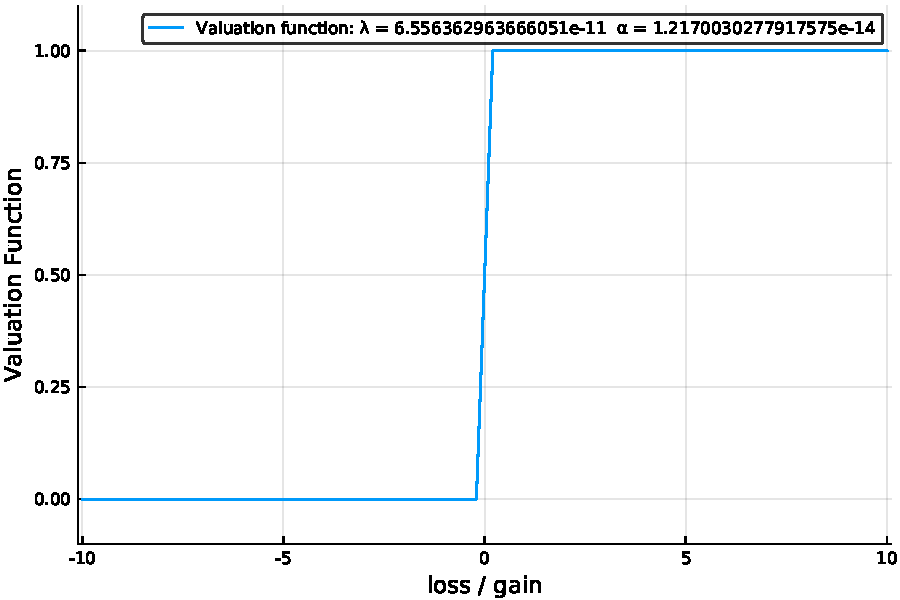
\includegraphics[width=.9\linewidth]{../Scripts/ValuationSingle.pdf}
\caption{\label{fig:single-valuation}Valuation function for all lotteries}
\end{figure}

\begin{figure}[htb]
\centering
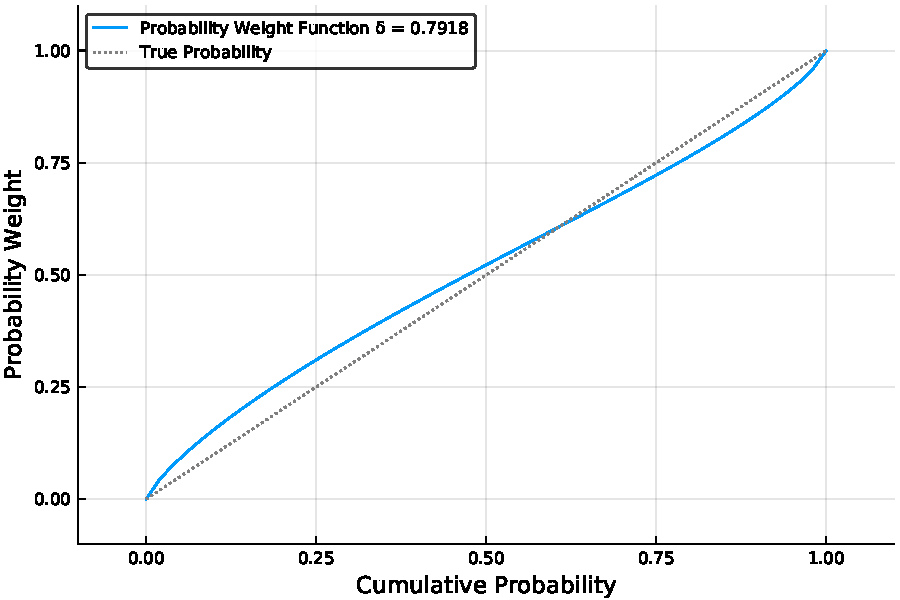
\includegraphics[width=.9\linewidth]{../Scripts/ProbWeightSingle.pdf}
\caption{\label{fig:single-prob}Probability Weighting Function for all lotteries}
\end{figure}

The most striking results from this is the shape of the valuation
function, which appears to approximate an indicator function. The
notion of loss-aversion that is usually assumed in the literature on
cumulative prospect theory is not apparent here, in fact, the opposite
is present. Consumers appear to not be affected at all by the
magnitude of losses, nor from the magnitude of the gains seen, only
seeming to care about the presence of a gain.

The Probability weighting function resembles the shape found by
Kahnmemann and Tversky, which had a $\delta$ of .65, the chief difference
being that it crosses the identity line at a higher cumulative
probability. This means that low-probability high-value items are
actually given less weight than Kahneman and Tversky suggest, which
goes contrary to my prior beliefs. It appears that the probabilities
are not that severely distorted, and although the relatively rare
probabilities are in fact overstated, the magnitude is not as immense
as one might expect in a lottery of this form.

One possible explanation for the lack of loss-aversion shown in this
data is the magnitude of the losses seen by the consumers. The current
price of many of the boxes is \$0.03, which indicates that many of the
losses can never have a magnitude of less than \$2.50. This is caused
by the fact that the items themselves can at smallest be valued at
\$0.03. In contrast the gains can be many magnitudes higher with some
items selling at upward of \$100.00. Since there is such a large
difference between possible gains and losses, consumers who are
particularly susceptible to confirmation bias may not value the losses
as they are low magnitude.

\subsection{Structural Differences between different lotteries}
\label{sec-5-1}

However, some boxes contain many more rare items than others. In
particular the cases titled \texttt{Chroma Case} and \texttt{Chroma Case 2} contain
many different rare items in many unique variants. These items are
quite valuable on the market, and there are many available in
the box. I tested to see if consumers behaved differently between
these boxes and the remaining boxes. The results are summarized below:

\begin{center}
\begin{tabular}{lll}
 & Chroma Case & Remaining Cases\\
Likelihood: &  & -2.388950505905629 x 10$^{\text{6}}$\\
$\lambda$ & 8.93682 x 10$^{\text{-55}}$ & 1.76366 x 10$^{\text{-14}}$\\
$\alpha$ & 0.486737 & 2.57372 x 10$^{\text{-10}}$\\
$\delta$ & 1.28239 & 0.774166\\
\end{tabular}
\end{center}

\begin{figure}[htb]
\centering
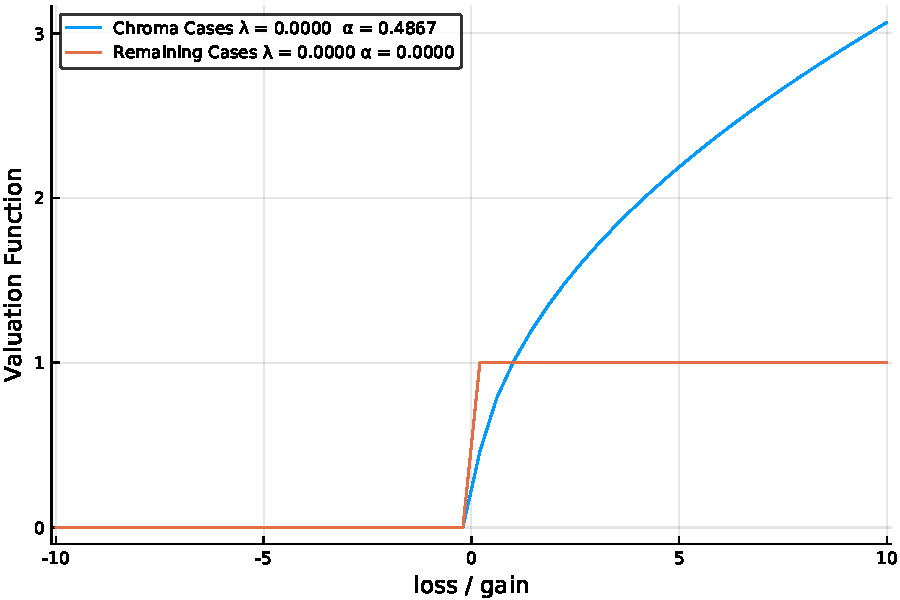
\includegraphics[width=.9\linewidth]{../Scripts/ValuationDual.pdf}
\caption{\label{fig:double-valuation}Valuation function for different lotteries}
\end{figure}

\begin{figure}[htb]
\centering
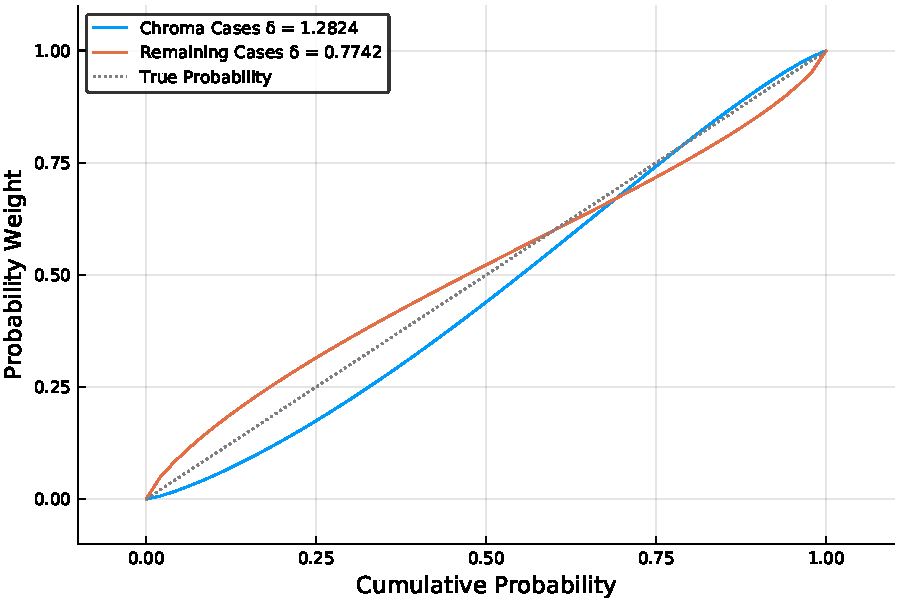
\includegraphics[width=.9\linewidth]{../Scripts/ProbWeightDual.pdf}
\caption{\label{fig:double-prob}Probability Weighting function for different lotteries}
\end{figure}

The first question to ask is whether or not these models are
significantly different from each other. Specifically, I am testing if
there is a difference between individual behaviors under the cases
containing many different items, and the cases containing many more
rare items. To this end I applied the likelihood ratio test against
the null hypothesis that there is no structural difference between the
two models. This led to a p-value of: 3.866 x 10$^{\text{-7}}$ . Under this
structure, there is a significant difference between the behavior of
individuals opening the chroma cases and the remaining cases.

Under both groups of data, loss aversion is simply not present. Using
a Wald statistic on the hypothesis that $\lambda$$_{\text{c}}$ = 0 and $\lambda$$_{\text{r}}$ = 0 gives a
probability that this did not occur from random noise of
7.107 x 10$^{\text{-52}}$, effectively a p-value of 1. This implies that
under the assumed structure of the model, there is simply no loss
aversion present. Whether or not this is caused by the structure
placed upon the model is not established, but I believe that the
framework is robust enough to preclude that possibility.

An interesting difference between these two models is the differences
in the $\alpha$ between the two structures. Since there are many more high
valuation items in the chroma cases, consumers are more sensitive to
higher valuations, as shown by the magnitude of the $\alpha$. This implies
that consumers are less convex in their valuations for the chroma
cases, as there are more high value items available, despite the same
probability of getting a very rare item.

The result that I found most perplexing however, was the value for $\delta$.
This value goes completely contrary to what cumulative prospect theory
predicts. As there are more high-value rare items available it
appears that less weight is applied to their probabilities. Applying a
Wald Test against the null hypothesis that $\delta$ < 1 yields a p-value of
0, implying that individuals are really not acting as predicted as
being risk seeking in low probability gains and risk averse in higher
probability gains. They appear to not weight the probabilities very
much at higher cumulative probabilities, overweighting the
probabilities of the middle-valued items, and under weighting the
probabilities of the very rare either in low or high value. One might
have expected that when there are more rare items, the probabilities
of these rare items would be overweighted rather than under weighted,
since the consumers are more sensitive to higher valuations, as shown
by the $\alpha$.

\subsection{Different reference dependence}
\label{sec-5-2}

In this section I consider the model if individuals consider gains and
losses as relative to the expected value of the crates and the price
they paid to open the crates. I changed the reference point to be the
price of the box, the price of the key, and the expected value of the
contents of the crate at the particular time. This changes the
viewpoint of the consumer: instead of viewing gains and losses as
relative to the initial income of the opener, we consider them as
gains and losses relative to what is expected to gain. Within this
paradigm a much different picture emerges.

\begin{center}
\begin{tabular}{lr}
Likelihood: & -2.389256828231863 x 10$^{\text{6}}$\\
$\lambda$ & 1.48236 x 10$^{\text{-11}}$\\
$\alpha$ & 0.0\\
$\delta$ & 0.108213\\
\end{tabular}
\end{center}

First we notice that the same results for $\lambda$ and $\alpha$ are present, that is
there is no loss aversion, and the valuation shape is approaching an
indicator function on whether or not it is a gain. However, the
probability weighting function has a much different value. This has
distorted its shape massively, lowering the function except for the
very high-value low-probability items.

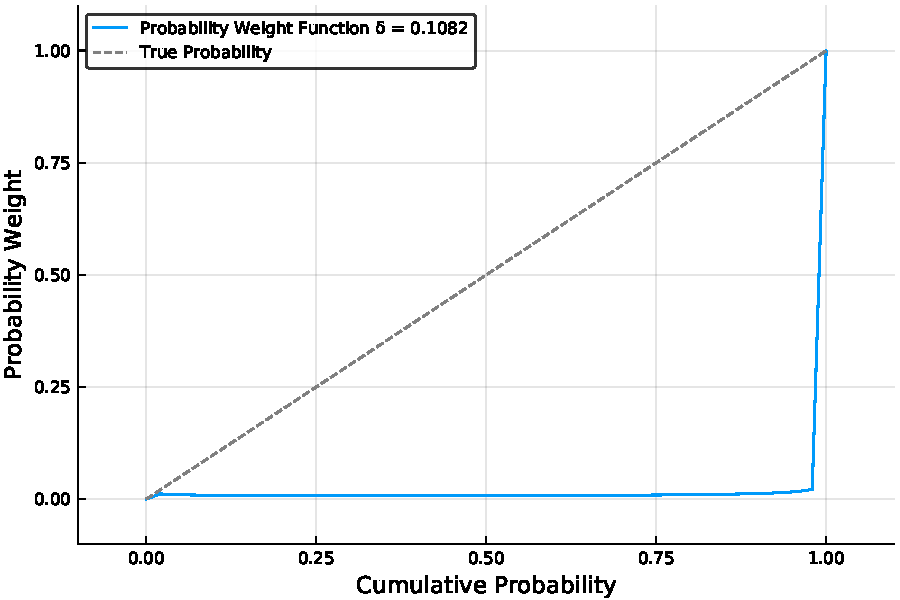
\includegraphics[width=.9\linewidth]{../Scripts/ProbWeightExpVal.pdf}

This begins to explain buying patterns in these crates, as it seems to
imply that the low value items do not matter at all, and that the very
rare items that have extremely low probabilities are massively
overweighted. This is consistent with the notion that only the very
rare high value items are driving the prices for the crates. It would
imply that losses opened from the crates are simply consolation
prizes, and their value is irrelevant. However I am reluctant to say
that this model fully explains the patterns of valuations because of
the lack of convexity of the valuation function, whose shape has not
changed. I believe that an extreme distortion of the probabilities is
occurring, as shown much more by this intrepretation of the structure
of the reference point. There are still aspects of the valuation not
explained by this particular form, nor by any form that I was able to
fit while maintaining the computational properties needed for
calculation.

\subsection{Further thoughts}
\label{sec-5-3}

While there is no way to investigate whether or not the data exhibits
reference dependence, as it is assumed under the structural
form. However, the fact that all specifications exhibit zero loss
aversion may be a powerful indicator that looking at total wealth
values may be the correct method to proceed in this context. If
consumers that are purchasing these items have a high level of wealth,
then small decreases in their income would have very little effect, as
represented in the data, and gains could have more of an effect,
especially if individuals engaging in these lotteries are
risk-loving. However, due to the lack of any covariate data available,
this is not something that can be tested in the current framework and
data, and is outside the scope of this paper.

It is difficult to test the predictive power of this model, since it
predicts valuations, and the vast majority of the data points are
censored. While in theory a test set of untested boxes could be
formed, and valuations for the box at each price level formed, and
then compared to the market price at that time, evaluating how close
to correct the data is would be difficult. Since a purchase only tells
us that the valuation was above the price, all that could be tested
was whether or not the valuation generated was above the price. This
is a poor metric for testing fit, and is a very difficult hurdle to
overcome. Looking explicitly at the buy orders is also not a random
sample of the valuations, as it is only the valuations that are above
the market price. As a result, I do not believe examining the
predictive power of this model on a test set is an effective way to
determine how well it describes valuations.

\section{Conclusions}
\label{sec-6}
The lack of more detailed data precludes many forms of complex
analysis, such as accounting for unobserved heterogeneity between
purchasers, or examining the extent at which current levels of income
affect behavior. Despite this, the data clearly shows that under
the structural assumptions of cumulative prospect theory, loss
aversion simply is not present. However it is impossible to say
whether the data is better described by this model than traditional
theory. One possibility for testing this would require data that is
simply not available for privacy reasons, such as covariates of wealth
or correlated variables. One alternative for further study is to data
mine the transaction history in the Steam Community Market, and view
the total value of the inventory of users who purchased. This would
allow for estimating wealth of the users; which would in turn be used
to test the assumption that lotteries are viewed in the context of
losses or gains rather than changes in wealth. However this would
require explicit permission from Valve as I believe it would be
invasive of users' privacy, and controlling for users that did not
allow for it would be pose problems with random sampling.

What the lack of loss aversion implies about consumer behavior is
interesting, as it either implies that the reference point of
consumers opening these boxes is not the price they pay, or that they
simply are not interested in instances when they incur a loss. There
is still a very small $\alpha$ value for many of the boxes, and changing the
reference point to be the price of the box, key and the expected value
of the crate does little to change this. These combined imply that the
lack of loss aversion is not explained by the reference point. The
valuation of the box seems to be driven by simply whether it makes a
loss or a gain rather than the degree. While there is an exception in
the cases that contain many rare items, whose value is driven by the
values of these rare items, the vast majority of the crates are not
driven by the individual item valuations, only whether or not there is
a gain. But even in the exception, since the probability weighting
function applies less weight to these rare events, it may be that this
structure explains the behavior of individuals facing
lotteries poorly, and exploring the avenues of expected utility theory would
give more insight into the valuations of consumers. This combined with
more powerful computation and structure may allow for a more robust
model of the valuations.

I do believe that a more robust model is required for properly
explaining the valuations seen in the data. While the computational
requirements of any more complicated model can be very high, allowing
for much more variation in the valuation function of individual
contents of the lotteries may better explain what is driving the
valuations of the entire lotteries. I find it hard to accept that the
valuation is driven simply by distortions of the probabilities and the
number of items that have positive valuations. Even if the distortions
are as extreme as predicted by the inclusion of the expected value in
the reference dependence, I do not believe that the an indicator
function properly describes the valuations. By requiring that the
valuations are viewed in the context of gains and losses, and imposing
convexity or concavity upon all gains and losses, virtually all of the
descriptive power of the model relies upon a proper border between
losses and gains being identified exogenously and correctly. However,
if it is chosen endogenously, possibly as expected value under the
probability weighting function's measure instead of the true
probabilities, it becomes extremely difficult to estimate the model. A
model that allowed for this change may have much more descriptive
power in a framework such as this.

\section{}
\label{sec-7}
\nocite{Efficiency}
\nocite{DoubleAuc}
\nocite{LimeBoy}
\nocite{LitReview}
\nocite{Liquidpedia}
\nocite{SteamMarket}

\bibliography{biblio}
% Emacs 25.3.1 (Org mode 8.2.10)
\end{document}